\title{
\centering

\includegraphics[width=4cm,height=4cm,keepaspectratio]{du.jpg} \\ \ CSE - 4255 Data Mining and Warehousing Lab\\  \Large \textit{Comparison Between the Performance of Decision Tree and Naive Bayes Classifier in Classification}\\}


\author{
        Saif Mahmud \\
        Roll: SH - 54\\
            \and
        M. Tanjid Hasan Tonmoy\\
        Roll: SH - 09\\
            \and
        \\\textbf{Submitted To:}\\ Dr. Chowdhury Farhan Ahmed \\
        Professor\\
        \\ \& \\ 
        Abu Ahmed Ferdaus\\
        Associate Professor\\ \\
        Department of Computer Science and Engineering\\
        University of Dhaka        
}
\date{\today}

\documentclass[12pt]{article}
\usepackage{graphicx}
\usepackage{cite}
\usepackage{url}
\usepackage{multirow}
\usepackage{longtable}
\usepackage{multirow}
%\usepackage[a4paper]{geometry}
\newcommand{\s}{\vspace{0.2cm}}
\usepackage{float}

\begin{document}


\maketitle
\thispagestyle{empty}
\clearpage
\newpage

\section{Problem Definition}
In this experiment, we have implemented two different classification algorithms, namely Decision tree and Naive Bayes. The algorithms utilize discrete and continuous features to predict class labels. Comparative analysis of these two algorithms have been conducted using various evaluation metrics for both balanced and imbalanced datasets of varied sizes.



\section{Theory}
\subsection{Decision Tree}
Decision tree learning is a supervised machine learning technique for inducing a decision tree from training data. A decision tree (also referred to as a classification tree or a reduction tree) is a predictive model which is a mapping from observations about an item to conclusions about its target value. In the tree structures, leaves represent classifications (also referred to as labels), non-leaf nodes are features, and branches represent conjunctions of features that lead to the classifications.

The algorithm is invoked with three parameters: D, attribute list, and Attribute selection method. We refer to D as a data partition. Initially, it is the complete set of training tuples and their associated class labels. The parameter attribute list is a list of attributes describing the tuples. Attribute selection method specifies a heuristic procedure for selecting the attribute that `best' discriminates the given tuples according to class. This procedure employs an attribute selection measure such as information gain or the Gini index. Whether the tree is strictly binary is generally driven by the attribute selection measure. Some attribute selection measures, such as the Gini index, enforce the resulting tree to be binary. Others, like information gain, do not, therein allowing multi-way splits (i.e., two or more branches to be grown from a node).

However, When a decision tree is built, many of the branches will reflect anomalies in the training data due to noise or outliers. Tree pruning methods address this problem of overfitting the data. Such methods typically use statistical measures to remove the least-reliable branches. Pruned trees tend to be smaller and less complex and, thus, easier to comprehend.


\subsection{Naive Bayes Classifier}
		
The Naive Bayesian classifier is based on Bayes’ theorem with the independence assumptions between predictors. A Naive Bayesian model is easy to build, with no complicated iterative parameter estimation which makes it particularly useful for very large datasets. Despite its simplicity, the Naive Bayesian classifier often does surprisingly well and is widely used because it often outperforms more sophisticated classification methods. Naive Bayesian classifiers assume that the effect of an attribute value on a given class is independent of the values of the other attributes. This assumption is called class-conditional independence. It is made to simplify the computations involved and, in this sense, is considered `naive'.

The goal of any probabilistic classifier is, with features $ x_0 $ through $ x_n $ and classes $ c_0 $ through $ c_k $, to determine the probability of the features occurring in each class, and to return the most likely class. Therefore, for each class, we want to be able to calculate P($ c_i $ | $ x_0 $, …, $ x_n $). In order to do this, we use Bayes rule. It may be noted that Bayes rule is the following:

$$ P(A \mid B) = \frac{P(B \mid A) \, P(A)}{P(B)} $$

\subsection{K - Fold Cross Validation}
In k-fold cross-validation, the initial data are randomly partitioned into k mutually exclusive subsets or `folds', $ D_1 $ , $ D_2 $ , . . . , $ D_k $ , each of approximately equal size. Training and testing is performed k times. In iteration i, partition $ D_i $ is reserved as the test set, and the remaining partitions are collectively used to train the model. That is, in the first iteration, subsets $ D_2 $ , . . . , $ D_k $ collectively serve as the training set to obtain a first model, which is tested on $ D_1 $ ; the second iteration is trained on subsets $ D_1 $ , $ D_3 $ , . . . , $ D_k $ and tested on $ D_2 $ ; and so on. Unlike the holdout and random subsampling methods, here each sample is used the same number of times for training and once for testing. For classification, the accuracy estimate is the overall number of correct classifications from the k iterations, divided by the total number of tuples in the initial data.

\section{Experimental Setup}
\subsection{Implementation}
For the implementation of decision tree, two different attribute selection methods (entropy and Gini index) have been used for both discrete and continuous attributes and is available as option for training models. hen there is a large number of distinct values for a continuous attribute, the training time increases significantly due to the fact that all possible splitting points have to be considered. The tree is stored using a dictionary structure in python and built recursively. Prepruning of the tree based on a threshold given as input has been used to prevent over-fitting.

In case of implementing Naive Bayes classifier, the prior and posterior probability is stored in the dictionary data structure in the training phase in order to ensure constant time retrieval during the prediction phase. The maximum likelihood estimates of probability for Bayesian rule is based on count in the case of categorical data and on the other hand, probability computed from Gaussian distribution in case of continuous data. To eradicate the zero probability due to sparse data, Laplace correction has been deployed in posterior probability calculation.  


 
\section{Result}
\subsection{Evaluation Metric}
The standard accuracy metric defined in (\ref{eqn:accuracy}) is used to evaluate the models used in this experiment.

\begin{equation}
\label{eqn:accuracy}
Accuracy = \frac{TP + TN}{TP + TN + FP + FN}
\end{equation} 

where, TP, TN, FP and FN are defined as True Positive, True Negative, False Positive and False Negative respectively. In this regard, true positive rate (TPR) or Recall or Sensitivity is defined as per the expression defined in (\ref{eqn:tpr}).

\begin{equation}
\label{eqn:tpr}
TPR / Recall / Sensitivity = \frac{TP}{TP + FN}
\end{equation} 

where, TP and FN are defined as True Positive and False Negative respectively.

On the other hand, Specificity and False Positive Rate (FPR) is specified as per (\ref{eqn:specificity}) and (\ref{eqn:fpr}) respectively.

\begin{equation}
\label{eqn:specificity}
Specificity = \frac{TN}{TN + FP}
\end{equation} 

\begin{equation}
\label{eqn:fpr}
FPR = 1 - Specificity
= \frac{TP}{TP + FN}
\end{equation} 

\begin{table}[H]
	\caption{Accuracy : Decision Tree}
	\centering
	\begin{tabular}{|c|c|c|}
		\hline
		\textbf{Dataset}  & \textbf{No of tuples} & \textbf{Accuracy \% {[}Entropy{]}} \\ \hline
		iris              & 150                   & 92.6607                            \\ \hline
		mushroom          & 8124                  & 98.5227                            \\ \hline
		breast cancer     & 286                   & 67.5955                            \\ \hline
		chess             & 3196                  & 66.0425                            \\ \hline
		connect-4         & 67557                 & 65.8303                            \\ \hline
		pendigits         & 7494                  & 19.469                             \\ \hline
		poker             & 1000000               & 50.1209                            \\ \hline
		creditcarddefault & 30000                 & 81.9945                            \\ \hline
		annealing         & 798                   & 77.2503                            \\ \hline
	\end{tabular}
\end{table}


% Please add the following required packages to your document preamble:
% \usepackage{multirow}
\begin{table}[H]
	\caption{Accuracy : Naive Bayes Classifier}
	\centering
	\begin{tabular}{|c|c|c|c|}
		\hline
		\textbf{Dataset}                     & \textbf{Dataset Size}   & \textbf{\begin{tabular}[c]{@{}c@{}}k-Fold Cross Validation\\ (k = 5) Accuracy (\%)\end{tabular}} & \textbf{Avg. Accuracy (\%)} \\ \hline
		\multirow{5}{*}{Adult}               & \multirow{5}{*}{32561}  & 82.9879                                                                                          & \multirow{5}{*}{83.35124}   \\ \cline{3-3}
		&                         & 83.2463                                                                                          &                             \\ \cline{3-3}
		&                         & 83.4459                                                                                          &                             \\ \cline{3-3}
		&                         & 83.6302                                                                                          &                             \\ \cline{3-3}
		&                         & 83.4459                                                                                          &                             \\ \hline
		\multirow{5}{*}{Breast Cancer}       & \multirow{5}{*}{286}    & 86.2069                                                                                          & \multirow{5}{*}{73.38174}   \\ \cline{3-3}
		&                         & 82.4561                                                                                          &                             \\ \cline{3-3}
		&                         & 64.9123                                                                                          &                             \\ \cline{3-3}
		&                         & 64.9123                                                                                          &                             \\ \cline{3-3}
		&                         & 68.4211                                                                                          &                             \\ \hline
		\multirow{5}{*}{Census-Income}       & \multirow{5}{*}{199523} & 85.6939                                                                                          & \multirow{5}{*}{85.57612}   \\ \cline{3-3}
		&                         & 85.255                                                                                           &                             \\ \cline{3-3}
		&                         & 85.5654                                                                                          &                             \\ \cline{3-3}
		&                         & 85.8235                                                                                          &                             \\ \cline{3-3}
		&                         & 85.5428                                                                                          &                             \\ \hline
		\multirow{5}{*}{Chess}               & \multirow{5}{*}{3196}   & 89.8438                                                                                          & \multirow{5}{*}{87.63982}   \\ \cline{3-3}
		&                         & 86.25                                                                                            &                             \\ \cline{3-3}
		&                         & 88.1064                                                                                          &                             \\ \cline{3-3}
		&                         & 88.7324                                                                                          &                             \\ \cline{3-3}
		&                         & 85.2665                                                                                          &                             \\ \hline
		\multirow{5}{*}{Chess - II}          & \multirow{5}{*}{28056}  & 36.2989                                                                                          & \multirow{5}{*}{36.2274}    \\ \cline{3-3}
		&                         & 36.545                                                                                           &                             \\ \cline{3-3}
		&                         & 36.1255                                                                                          &                             \\ \cline{3-3}
		&                         & 36.3361                                                                                          &                             \\ \cline{3-3}
		&                         & 35.8315                                                                                          &                             \\ \hline
		\multirow{5}{*}{Connect-4}           & \multirow{5}{*}{67557}  & 72.1137                                                                                          & \multirow{5}{*}{72.15832}   \\ \cline{3-3}
		&                         & 72.7353                                                                                          &                             \\ \cline{3-3}
		&                         & 72.2617                                                                                          &                             \\ \cline{3-3}
		&                         & 71.7786                                                                                          &                             \\ \cline{3-3}
		&                         & 71.9023                                                                                          &                             \\ \hline
		\multirow{5}{*}{Credit Card Default} & \multirow{5}{*}{30000}  & 67.2055                                                                                          & \multirow{5}{*}{65.12984}   \\ \cline{3-3}
		&                         & 70.4167                                                                                          &                             \\ \cline{3-3}
		&                         & 53.0167                                                                                          &                             \\ \cline{3-3}
		&                         & 73.2167                                                                                          &                             \\ \cline{3-3}
		&                         & 61.7936                                                                                          &                             \\ \hline
		\multirow{5}{*}{Iris}                & \multirow{5}{*}{150}    & 93.3333                                                                                          & \multirow{5}{*}{95.33334}   \\ \cline{3-3}
		&                         & 90                                                                                               &                             \\ \cline{3-3}
		&                         & 96.6667                                                                                          &                             \\ \cline{3-3}
		&                         & 96.6667                                                                                          &                             \\ \cline{3-3}
		&                         & 100                                                                                              &                             \\ \hline
	\end{tabular}
\end{table}
% Please add the following required packages to your document preamble:
% \usepackage{multirow}
\begin{table}[H]
	\begin{tabular}{|c|c|c|c|}
		\hline
		\textbf{Dataset}           & \textbf{Dataset Size}    & \textbf{\begin{tabular}[c]{@{}c@{}}k-Fold Cross Validation\\ (k = 5) Accuracy (\%)\end{tabular}} & \textbf{Avg. Accuracy (\%)} \\ \hline
		\multirow{5}{*}{Mushroom}  & \multirow{5}{*}{8124}    & 95.326                                                                                           & \multirow{5}{*}{95.37192}   \\ \cline{3-3}
		&                          & 95.0154                                                                                          &                             \\ \cline{3-3}
		&                          & 94.4                                                                                             &                             \\ \cline{3-3}
		&                          & 95.6281                                                                                          &                             \\ \cline{3-3}
		&                          & 96.4901                                                                                          &                             \\ \hline
		\multirow{5}{*}{Pendigits} & \multirow{5}{*}{7494}    & 78.7333                                                                                          & \multirow{5}{*}{78.0755}    \\ \cline{3-3}
		&                          & 78.6                                                                                             &                             \\ \cline{3-3}
		&                          & 77.7333                                                                                          &                             \\ \cline{3-3}
		&                          & 77.5183                                                                                          &                             \\ \cline{3-3}
		&                          & 77.7926                                                                                          &                             \\ \hline
		\multirow{5}{*}{Poker}     & \multirow{5}{*}{1000000} & 50.119                                                                                           & \multirow{5}{*}{50.1187}    \\ \cline{3-3}
		&                          & 50.114                                                                                           &                             \\ \cline{3-3}
		&                          & 50.12                                                                                            &                             \\ \cline{3-3}
		&                          & 50.1205                                                                                          &                             \\ \cline{3-3}
		&                          & 50.12                                                                                            &                             \\ \hline
		
		\multirow{5}{*}{\begin{tabular}[c]{@{}c@{}}Breast Cancer - \\ Wisconsin\end{tabular}} & \multirow{5}{*}{699}  & 65.035                                                                                           & \multirow{5}{*}{62.78208}   \\ \cline{3-3}
		&                       & 63.8298                                                                                          &                             \\ \cline{3-3}
		&                       & 62.4113                                                                                          &                             \\ \cline{3-3}
		&                       & 60.8696                                                                                          &                             \\ \cline{3-3}
		&                       & 61.7647                                                                                          &                             \\ \hline
	\end{tabular}
\end{table}


\begin{table}[H]
	\caption{Dataset : Adult}
	\centering
	\begin{tabular}{|c|c|c|c|}
		\hline
		\textbf{Class Label} & \textbf{Precision} & \textbf{Recall} & \textbf{F1-Score} \\ \hline
		\textless{}=50K      & 0.85               & 0.93            & 0.89              \\ \hline
		\textgreater{}50K    & 0.7                & 0.5             & 0.58              \\ \hline
		\textbf{Avg}         & 0.82               & 0.83            & 0.82              \\ \hline
	\end{tabular}
\end{table}

\begin{table}[H]
	\caption{Dataset : Breast Cancer}
	\centering
	\begin{tabular}{|c|c|c|c|}
		\hline
		\textbf{Class Label} & \textbf{Precision} & \textbf{Recall} & \textbf{F1-Score} \\ \hline
		no-recurrence-events & 0.75               & 0.82            & 0.79              \\ \hline
		recurrence-events    & 0.46               & 0.35            & 0.4               \\ \hline
		\textbf{Avg}         & 0.66               & 0.68            & 0.67              \\ \hline
	\end{tabular}
\end{table}

\begin{table}[H]
	\caption{Dataset : PenDigit}
	\centering
	\begin{tabular}{|c|c|c|c|}
		\hline
		\textbf{Class Label} & \textbf{Precision} & \textbf{Recall} & \textbf{F1-Score} \\ \hline
		0                    & 0.96               & 0.93            & 0.94              \\ \hline
		1                    & 0.77               & 0.83            & 0.80              \\ \hline
		2                    & 0.90               & 0.93            & 0.91              \\ \hline
		3                    & 0.81               & 0.92            & 0.86              \\ \hline
		4                    & 0.00               & 0.00            & 0.00              \\ \hline
		5                    & 0.58               & 0.60            & 0.59              \\ \hline
		6                    & 0.99               & 0.97            & 0.98              \\ \hline
		7                    & 0.99               & 0.90            & 0.94              \\ \hline
		8                    & 0.82               & 0.92            & 0.87              \\ \hline
		9                    & 0.48               & 0.90            & 0.63              \\ \hline
		\textbf{avg}         & 0.73               & 0.79            & 0.75              \\ \hline
	\end{tabular}
\end{table}


\begin{figure}[H]
	\centering
	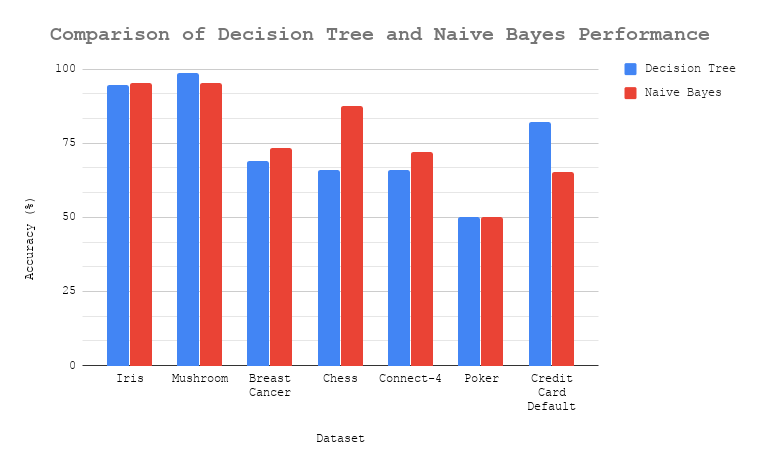
\includegraphics[width = \columnwidth, height = 9.5cm]{Comparison.png}
	\caption{Comparison between Decision Tree and Naive Bayes}
	\label{fig:comparison}
\end{figure}


\section{Discussion}
Both of these algorithms produce reasonable performance when dealing with moderate sized datasets with close to balanced class distribution. However, in case of class imbalance, both of thee algorithms suffer. The insights we have obtained through the experiment on aforementioned classification algorithm is given below:

\begin{itemize}
	\item In case of highly imabalanced dataset with very few positive or negative example, the classifier overfits the dominant class in most of the cases. Therefore, we can see in Figure \ref{fig:BreastCancerWisconsin} that only the dominant class has been detected correctly in the diagonal position with very few precise classification for the scarce class labels.


\begin{figure}[H]
	\centering
	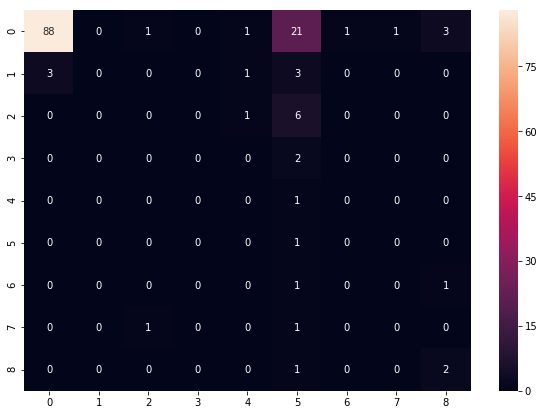
\includegraphics[width = .7\columnwidth, height = 7.5cm]{BreastCancerWisconsin.png}
	\caption{Confusion Matrix - Breast Cancer Wisconsin}
	\label{fig:BreastCancerWisconsin}
\end{figure}

\item In the scenario of multi-class classification with many classes in comparison with the number of tuples in the dataset, both decision tree and naive bayes classifier tends to fail in segmenting with higher accuracy which is depicted in Figure \ref{fig:chess2}.  

\begin{figure}[H]
	\centering
	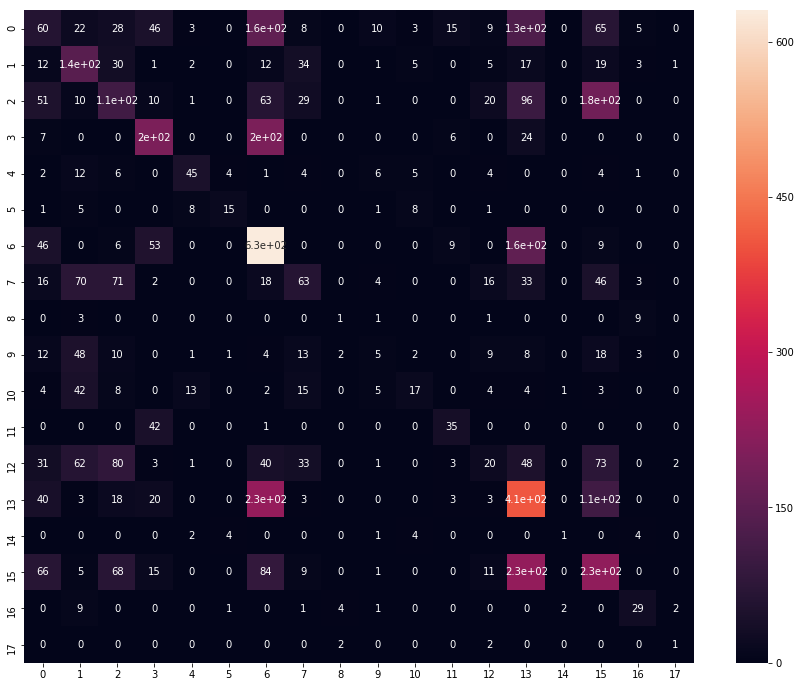
\includegraphics[width = 0.9\columnwidth, height = 8.5cm]{Chess_II.png}
	\caption{Confusion Matrix - Chess II}
	\label{fig:chess2}
\end{figure}

\item With balanced distribution of multiple classes and reasonable amount of training tuples representing dataset size, the classification algorithms performs reasonably well which is evident in the diagonal entries of Figure \ref{fig:pendigit}.

\begin{figure}[H]
	\centering
	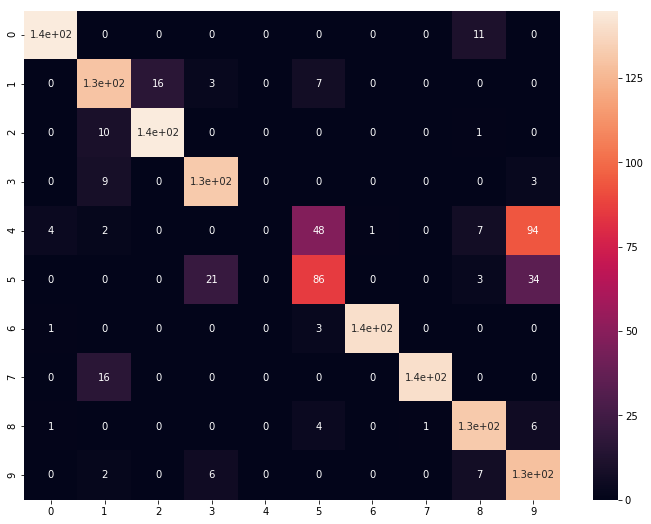
\includegraphics[width = .7\columnwidth, height = 7.5cm]{PenDigit.png}
	\caption{Confusion Matrix - PenDigit}
	\label{fig:pendigit}
\end{figure}
\end{itemize}

\end{document}
